\documentclass{article}

\usepackage[final]{neurips_2019}

\usepackage[utf8]{inputenc}
\usepackage[T1]{fontenc}
\usepackage{hyperref}
\usepackage{url}
\usepackage{booktabs}
\usepackage{amsfonts}
\usepackage{nicefrac}
\usepackage{microtype}
\usepackage{graphicx}
\usepackage{amsmath}  
\usepackage{xcolor}
\usepackage{lipsum}

\newcommand{\note}[1]{\textcolor{blue}{{#1}}}

\title{
  Transferability of counterfactual examples across different models\\
  \vspace{1em}
  \small{\normalfont Project Work - Responsible AI (by Bilal Zafar)}
}

\author{
  Frederik Hüttemann \\
  Applied Computer Science\\
  Ruhr-Universität Bochum \\
  \texttt{frederik.huettemann@rub.de} \\
}

\begin{document}

\maketitle

\begin{abstract}
Neural networks and other machine learning models are increasingly being used in sensitive areas of application such as criminal justice or healthcare. It is essential to make their decisions comprehensible. Counterfactual examples (CEs) provide a way to explain a model's decisions by showing how input data would need to be changed to achieve a different prediction. CEs are usually considered model-specific, which limits their practical applicability.\\
The aim of this work is to investigate the transferability of CEs between different models. To this end, two central experiments were conducted: In the first, reference models with identical architecture but different number of training epochs were compared. In the second experiment, the model complexity varied. The experiments were performed on both tabular data (COMPAS, ACS) and image data (MNIST, Fashion MNIST, CIFAR-10, ImageNet) with different model types (FFNN, CNN, Random Forest, SVM). \\
The results show that CEs are transferable under certain conditions. For neural networks, a significant negative correlation was found between transferability rate and both training duration and model complexity. In contrast, random forest models showed a positive correlation. Overall, the project work confirms that CEs can be transferable in principle. However, the transferability rate strongly depends on the data type and model used.\\

\end{abstract}

\section{Introduction}
Counterfactual examples (CE) are a method to explain a model's decision by showing how one or more input features would have to change in order to have a different model output. This explainability method is often used in life-critical domains, such as healthcare or criminal justice, where a binary classification task is performed. For example, in criminal justice, a model might predict whether a defendant will reoffend within two years. \\
The generation of CEs is typically model-specific, as it generally only applies to a particular model. In this project, it is investigated whether CEs for the base model also work for different models or if they are model-specific. This is done by gradually increasing the difference between the base model and the reference model. In the first experiment two models only differ in the number of training epochs. In the other experiment the number of layers and hidden units is different. The goal is to find trends in the transferability of CEs across different models, formulate them as hypotheses and formally proof them. \\
For the experiments two different types of data are used: tabular data and image data. Using multiple different datasets allows to reliably find trends and proof or disproof the hypotheses. On the tabular data, simple feed-forward neural networks (FFNN), Random Forest (RF) and kernelized SVM (K-SVM) are used, while on the image data more complex convolutional neural networks (CNN) are used. \\

\section{Related Work}
CEs are a well-known method to explain the decisions of a model. Machine learning is used in many different domains, such as healthcare, job applications and administrative decisions. In these domains, it is important to understand the model's decisions and to be able to explain them. Using CEs, a user can understand how the model's decision would change if one or more input features were changed. This is especially important in life-critical domains, where wrong decisions can have severe consequences. \cite{examples_cf_applications}\\
Normally, the generation of CEs is input specific which means that the algorithm needs a specific data point for which the opposite should be predicted. However, there are approaches to generate more general, diverse and feasible CEs, which do not rely on a specific datapoint as input. A set of them can be used to understand local model behavior and approximate the decision boundary at a given point. \cite{examples_cf_applications} \\
It is stated that CEs are closely linked to adversarial examples which can be used to attack a model by generating inputs that are misclassified. This is done by changing the input features in a way that the model's decision changes. Same rule applies for CEs. The key difference is, that a CE is optimized to be classified into a specific class, while adversarial examples are designed to mislead models in general. An approach is developed which allows attacks on unknown models by using adversarial examples generated on a known model. They managed to generated general adversarial examples that lead to a high number of misclassifications. \cite{papernot2016transferabilitymachinelearningphenomena} \\

\section{Approach}
In the related work section, it is stated that CEs are often model-specific and therefore cannot be transferred across different models. However, it is also known that adversarial examples, which are are similar to CEs, can be used to attack unknown different models.\\
In this project, experiments are done to find out whether CEs can be transferred. For this, two simple experiments are designed to highlight trends. For each experiment, a hypothesis is formulated which should be proven. Using multiple different datasets and different type of models, averages can be calculated on which the hypothesis can be tested.\\
In general, every experiment utilizes two models. The first model is called the \textit{base model} and is used to generate CEs. The second model is called the \textit{reference model} and is used to evaluate the transferability of the CEs. Both models are trained on the same data to ensure that the CEs are not biased towards a specific model.\\

\section{Experiments}
The experiments, which are described in this section, are designed to find trends in the transferability of CEs. For simplicity, only binary classification is considered. To solve a binary classification task, different types of models can be used. Here, FFNN, CNN, RF, K-SVM are evaluated as these are commonly used architectures. For neural networks the generation of counterfactual examples is based on gradient-methods. RF and K-SVM are not differentiable, so for these models the DiCE library is used \cite{dice_cf}. This approach relies on a loss function which is also optimized using gradient descent. It combines the distance between the original input and the distance to the counterfactual class while maintaining diversity in the generated counterfactuals. \\
\begin{equation}
    \text{transferability rate} = \frac{\text{CEs classified in counterfactual class}}{\text{total number of CEs}}
    \label{eq:transferability_rate}
    \vspace{0.5cm}
\end{equation}
\noindent
To evaluate the transferability of CEs, a metric is needed that quantifies how well the CEs transfer to the reference model. This metric is called the \textit{transferability rate}. The transferability rate is given by equation \ref{eq:transferability_rate} and is defined as the ratio of the number of CEs that are correctly classified in the counterfactual class by the reference model to the total number of CEs generated by the base model. The transferability rate is a value between 0 and 1, where 0 means that none of the CEs are correctly classified in the counterfactual class by the reference model and 1 means that all CEs are correctly classified in the counterfactual class.\\
Because the training and generation of CEs is computational expensive, the transferability rate is only calculated for a limited number (250) of CEs. Eventough this number is low, the later presented results show that the number is sufficient to find trends in the transferability of CEs as well as to formulate and proof hypotheses. The transferability rate is calculated for each experiment and for each model.\\
To find trends in the transferability of CEs, the idea was to start as simple as possible and then gradually increase the complexity of the experiments. Each experiment is done for multiple iterations to ensure that randomness does not influence the results. Each resulting datapoint is an average over the different runs.

\subsection{Experiment 1: Base model vs. reference model with different number of epochs}
The first experiment is designed very simple. Here, both the base model and the reference model have the same model architecture. The base model is trained for a fixed number of epochs (here 10 epochs) on the training data. The reference model is a copy of the trained base model, but its training is continued for additional epochs. For additional epoch zero, the base model and the reference model are identical. Here, the transferability rate should be one. As the number of additional epochs increases, the transferability rate should decrease as the reference model's weights are updated and differ more and more from the base model's weights. Therefore the reference model's decision boundary is updated and the CEs generated by the base model are not necessarily classified in the counterfactual class by the reference model anymore. 
The hypothesis for this experiment is:
\begin{itemize}
    \item \textbf{Hypothesis 1:} The transferability rate decreases as the number of additional epochs increases.
\end{itemize}
It is important to note, that this experiment can only be performed on models, which rely on gradient descent to update their weights as they are trained for a fixed number of epochs. RF and K-SVM at some point do convergence and then are not updated anymore. \\
The test is run on all types of data. For the tabular data FFNNs and for image data CNNs are used. Apart from multiple test iterations different hyperparameters for the models are also used to reduce bias.

\subsection{Experiment 2: Base model vs. reference model with different number of parameters}
The second experiment is similar to the first one. Again the base model and the reference model are the same model architecture and trained with the same hyperparameters. The only difference is that the models both trained from scratch and therefore differ in their initialization. As the random initialization of the weights is different, the models learn different decision boundaries. The more parameters the model has, the more complex the decision boundary can be. Two models with a high number of parameters probably learn different decision boundaries and therefore have a lower transferability rate than two models with a low number of parameters. The hypothesis for this experiment is:
\begin{itemize}
    \item \textbf{Hypothesis 2:} The transferability rate decreases as the model's complexity increases.
\end{itemize}
To test this hypothesis, the experiments are performed with different model architectures and different type of data. It is also important to note, that the model's complexity needs a metric for every architecture. For the FFNN, the number of linear layers is choosen as a quantifier for the complexity. CNNs consist of two major parts: the convolutional layers and the linear layers. As it is not intuitive to quantify the complexity using convolutional layers, for CNNs the number of total features in the linear layer part has been taken as an indicator for complexity. For RF the maximum allowed tree depth and for K-SVM the polynomial degree is choosen.

\subsection{Data}
The used data can be divided into two categories: tabular data and image data. For the tabular data, two datasets are used: a \textit{COMPAS} dataset \cite{compas_dataset} and an \textit{ACS} dataset \cite{acs_dataset}. \\
The \textit{COMPAS} dataset contains information about criminal defendants, such as their age, the prior number of offenses, and the type of offense. The goal is to predict whether a defendant will reoffend within two years. \\
The \textit{ACS} dataset contains information about the American Community Survey, such as the age, education, and income of individuals. The dataset label is whether the the data point represents a person who is employed or not. \\
For image classification data there are many different possible datasets to choose from. As only a binary classification tasks are considered, the datasetss had to be converted into a binary classification task. The used datasets are \textit{CIFAR-10} \cite{cifar10_dataset}, \textit{Imagenet} \cite{imagenet_dataset}, \textit{MNIST} \cite{mnist_dataset} and \textit{Fashion MNIST} \cite{fashion_mnist}.\\
\textit{MNIST} and \textit{Fashion MNIST} are both low resolution (28x28 pixels) grayscale images of handwritten digits and clothing items. It contains 10 classes, one for each digit or clothing item. To convert it to a binary classification task, every datapoint representing a \textit{digit 0} becomes a positive example, while all other datapoints become negative examples. \\
For \textit{CIFAR-10}, the images are also low resolution (32x32 pixels) but colored. Similar to \textit{MNIST}, the positive class is \textit{airplane} and the negative class is everything else. \\
The same approach has been taken for \textit{Imagenet}, where the images are high resolution (224x224 pixels), colored images and representing 1000 classes. The positive class is \textit{orange} and the negative class is everything else. Here, the positive and negative examples are balanced, so that the number of positive and negative examples is equal. The selection of the images for the rest class is done by randomly selecting images from the other classes. \\
The datasets are split into a training set and a test set. The training set is the same for all experiments, the test set is on the one hand used to evaluate and compare models but also to generate CEs. This way, the CEs are not biased towards a specific model because they are generated on the same, new unknown test data. 

\subsection{Evaluation method}
The evaluation method is based on the transferability rate, which is defined in equation \ref{eq:transferability_rate}. Because multiple datapoints correspond to one result, the averages are taken. This way outliers in the experiments are only partially taken into account.\\
To identify trends, a linear interpolation line is calculated. \\
To verify the stated hypotheses, the Spearman rank correlation coefficient is calculated. The Spearman rank correlation coefficient is a measure of correleation between two variables. It is used to determine whether there is a monotonic relationship between the two variables. The Spearman rank correlation coefficient is a value between -1 and 1, where -1 means that there is a perfect negative correlation, 0 means that there is no correlation and 1 means that there is a perfect positive correlation. The hypotheses can be confirmed or rejected by also calculating the p-value. The p-value is a measure of the statistical significance of the correlation. As a common threshold for statistical significance, a p-value of 0.05 is used. If the p-value is below this threshold, the hypothesis is confirmed, otherwise it is rejected. \cite{spearman_rank_correlation}\\

\section{Results}
\subsection{Experiment 1: Base model vs. reference model with different number of epochs}
The evaluation of the first experiment is only based on neural networks as they do include epoch-wise training. For a better overview, the results of image and tabular data is split. Figure \ref{fig:add_epochs_image} shows the average transferability rate for additional training epochs on different image datasets. The used model architecture is a CNN with two to four convolutional layers followed by two linear layers.\\
\begin{figure}[h]
    \centering
    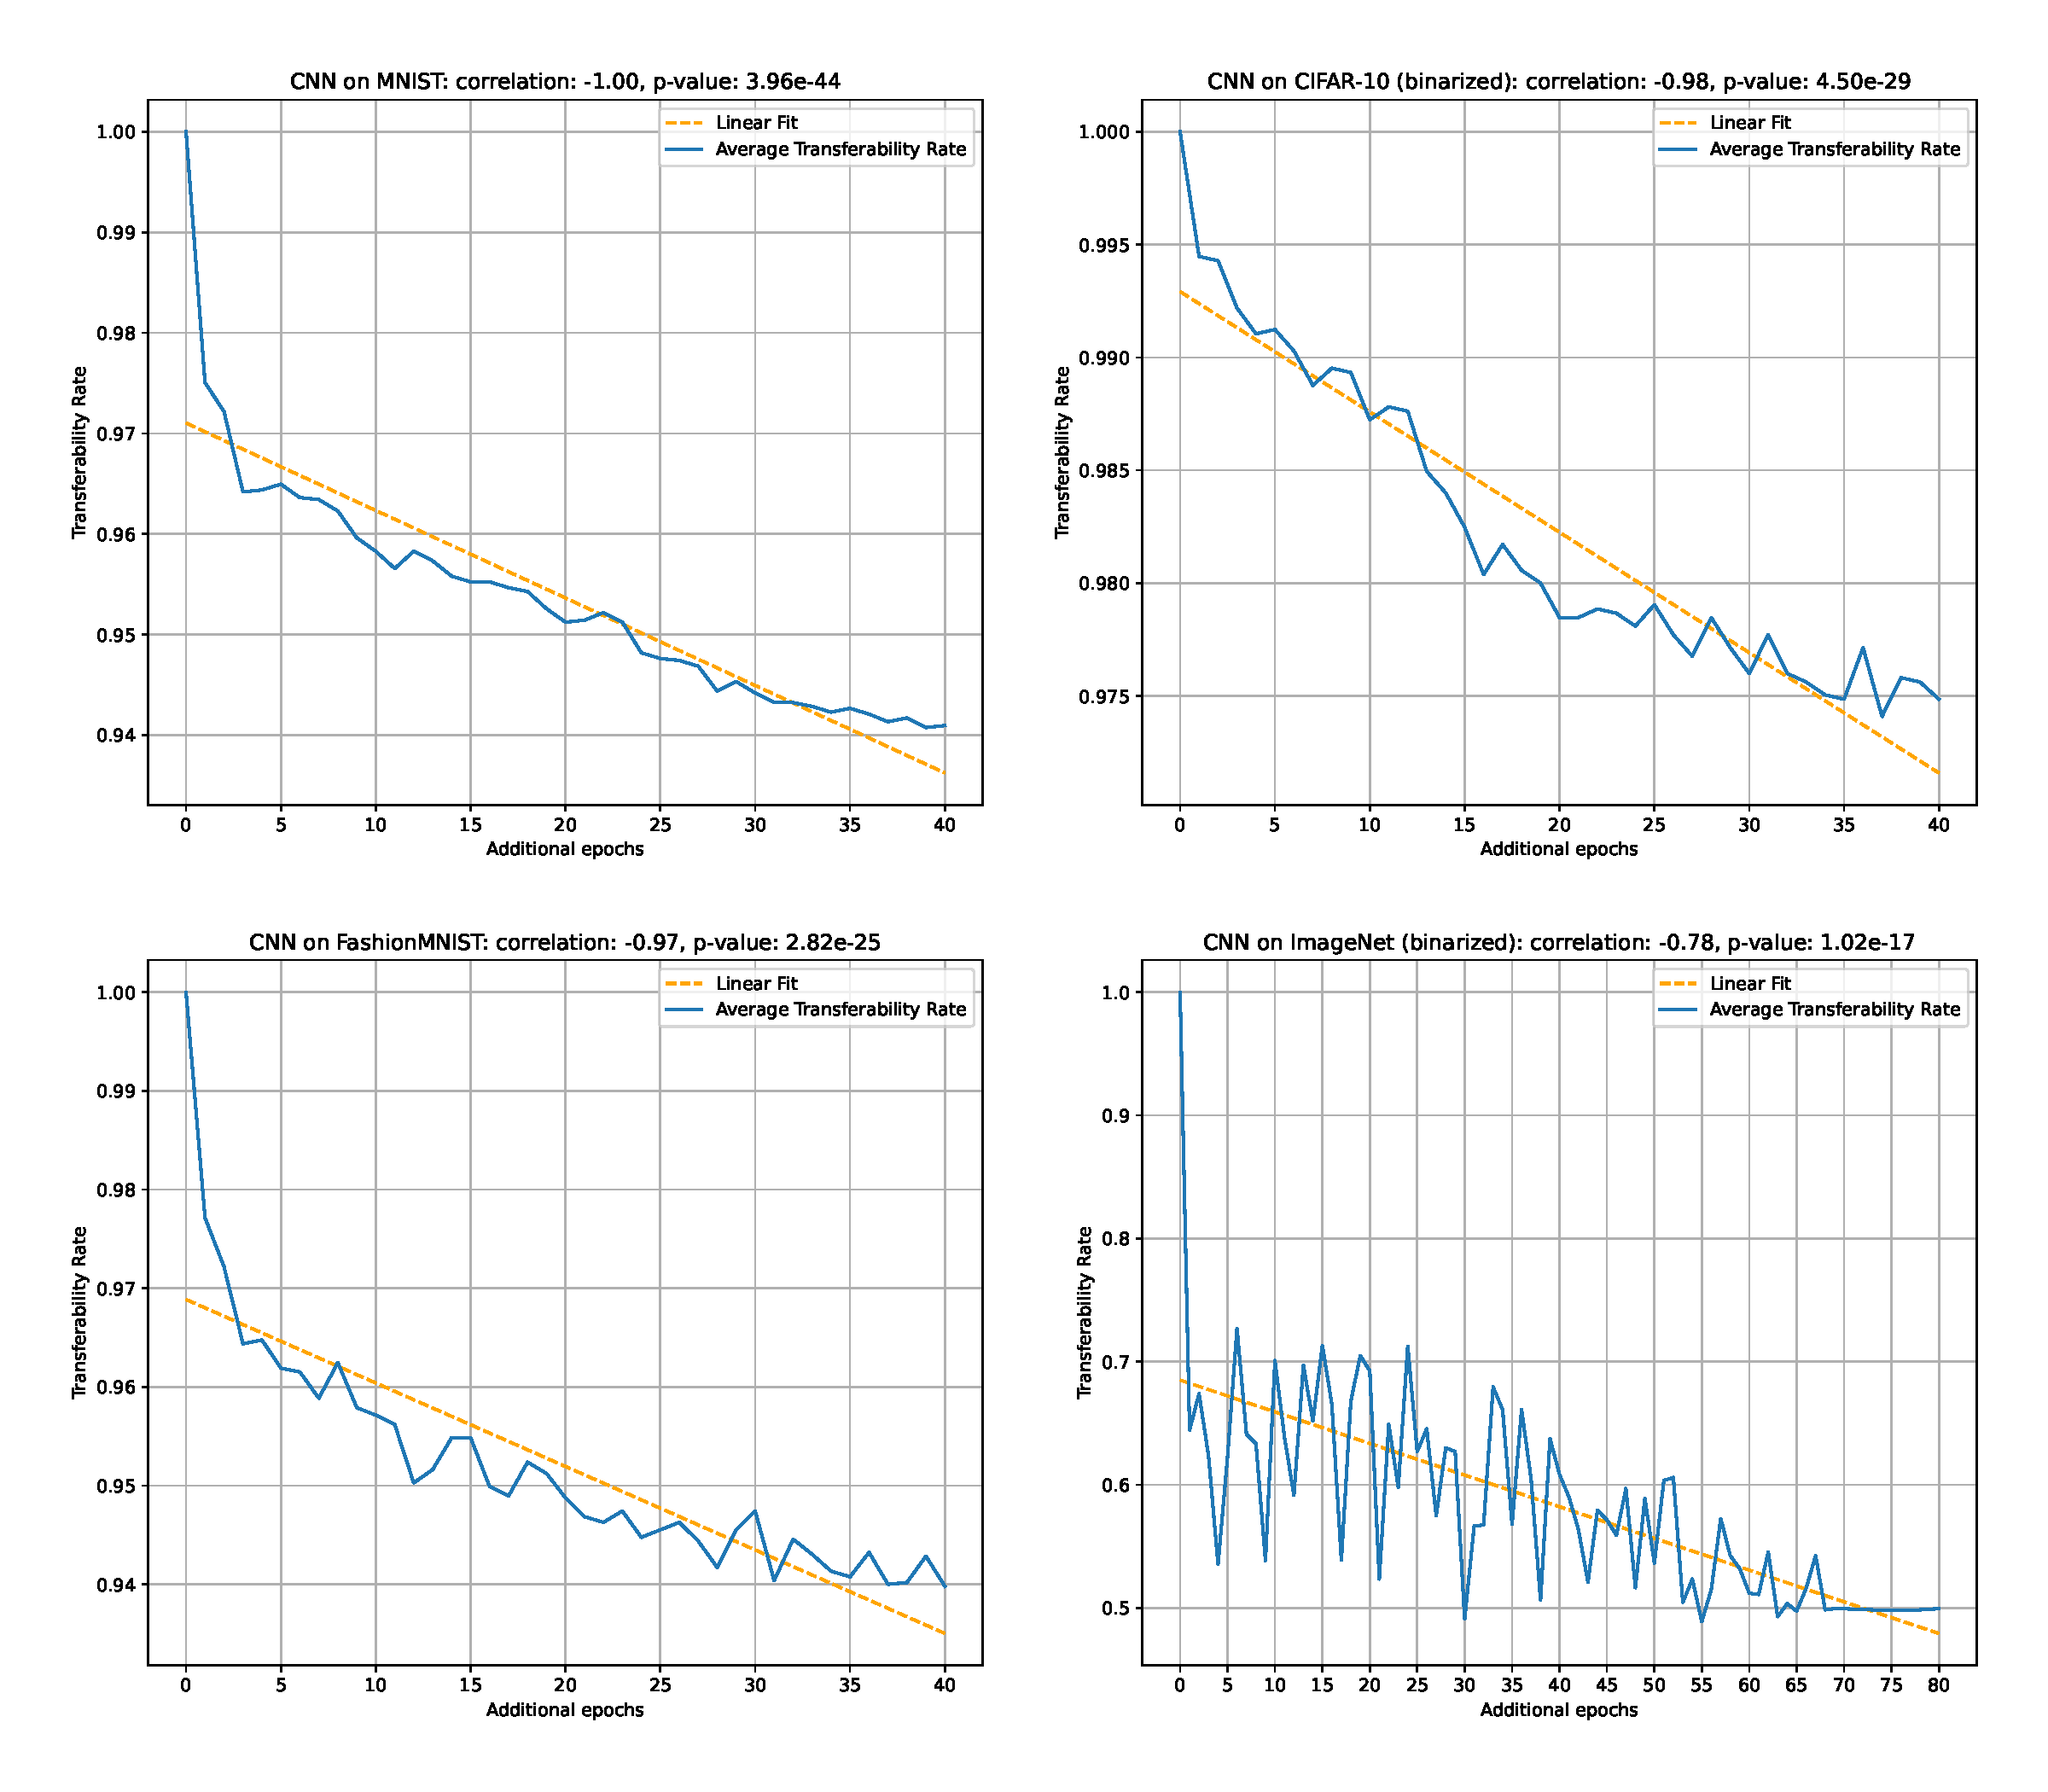
\includegraphics[width=\linewidth]{abb/epoch_evaluation_image.pdf}    
    \caption{Average transferability rate for additional training epochs on image datasets. CNNs were evaluated with different hyperparameters for number of layers and number of features to have a higher number of sampels.}    
    \label{fig:add_epochs_image}    
\end{figure}
\noindent
For every image dataset a similar trend can be observed. The transferability rate decreases with additional training epochs. To emphasize the trend, the linear interpolation line is drawn. All rates start at a value of $1$ for no additional epochs. For the both \textit{MNIST} datasets, the average transferability rate after 40 epochs is still above 94 \%. For the binarized \textit{CIFAR-10} the transferability rate is approximatly 97.5 \% after 40 additional training epochs. The only outlier in the image datasets is the experiment on the \textit{ImageNet} dataset. Here, the transferability rate drops to 65 \% after the first additional training epoch and fluctuates a lot around this value. With more training epochs, the rate decays to 50 \%. Because the high and low peaks of the graph, a higher number of training epochs has been taken for this experiment, to emphasize the dependency. However, a negative correlation can still be observed.\\
Figure \ref{fig:examples_image} shows an example image for each image dataset. The counterfactual images for \textit{MNIST} and \textit{Fashion MNIST} did only change the constrast a bit. The black background is a bit lighter while the white is a bit darker. For the \textit{CIFAR-10} example, there is no visible difference between the original and counterfactual image. The CE for the \textit{ImageNet} dataset show, why the transferability rate immediately drops after a single epoch of training. Because these images are high resolution images, only minimal artifacts can be seen in red. This results in fewer CEs which are transferable as these artifacts probably are very model-specific.\\
\begin{figure}[h]
    \centering
    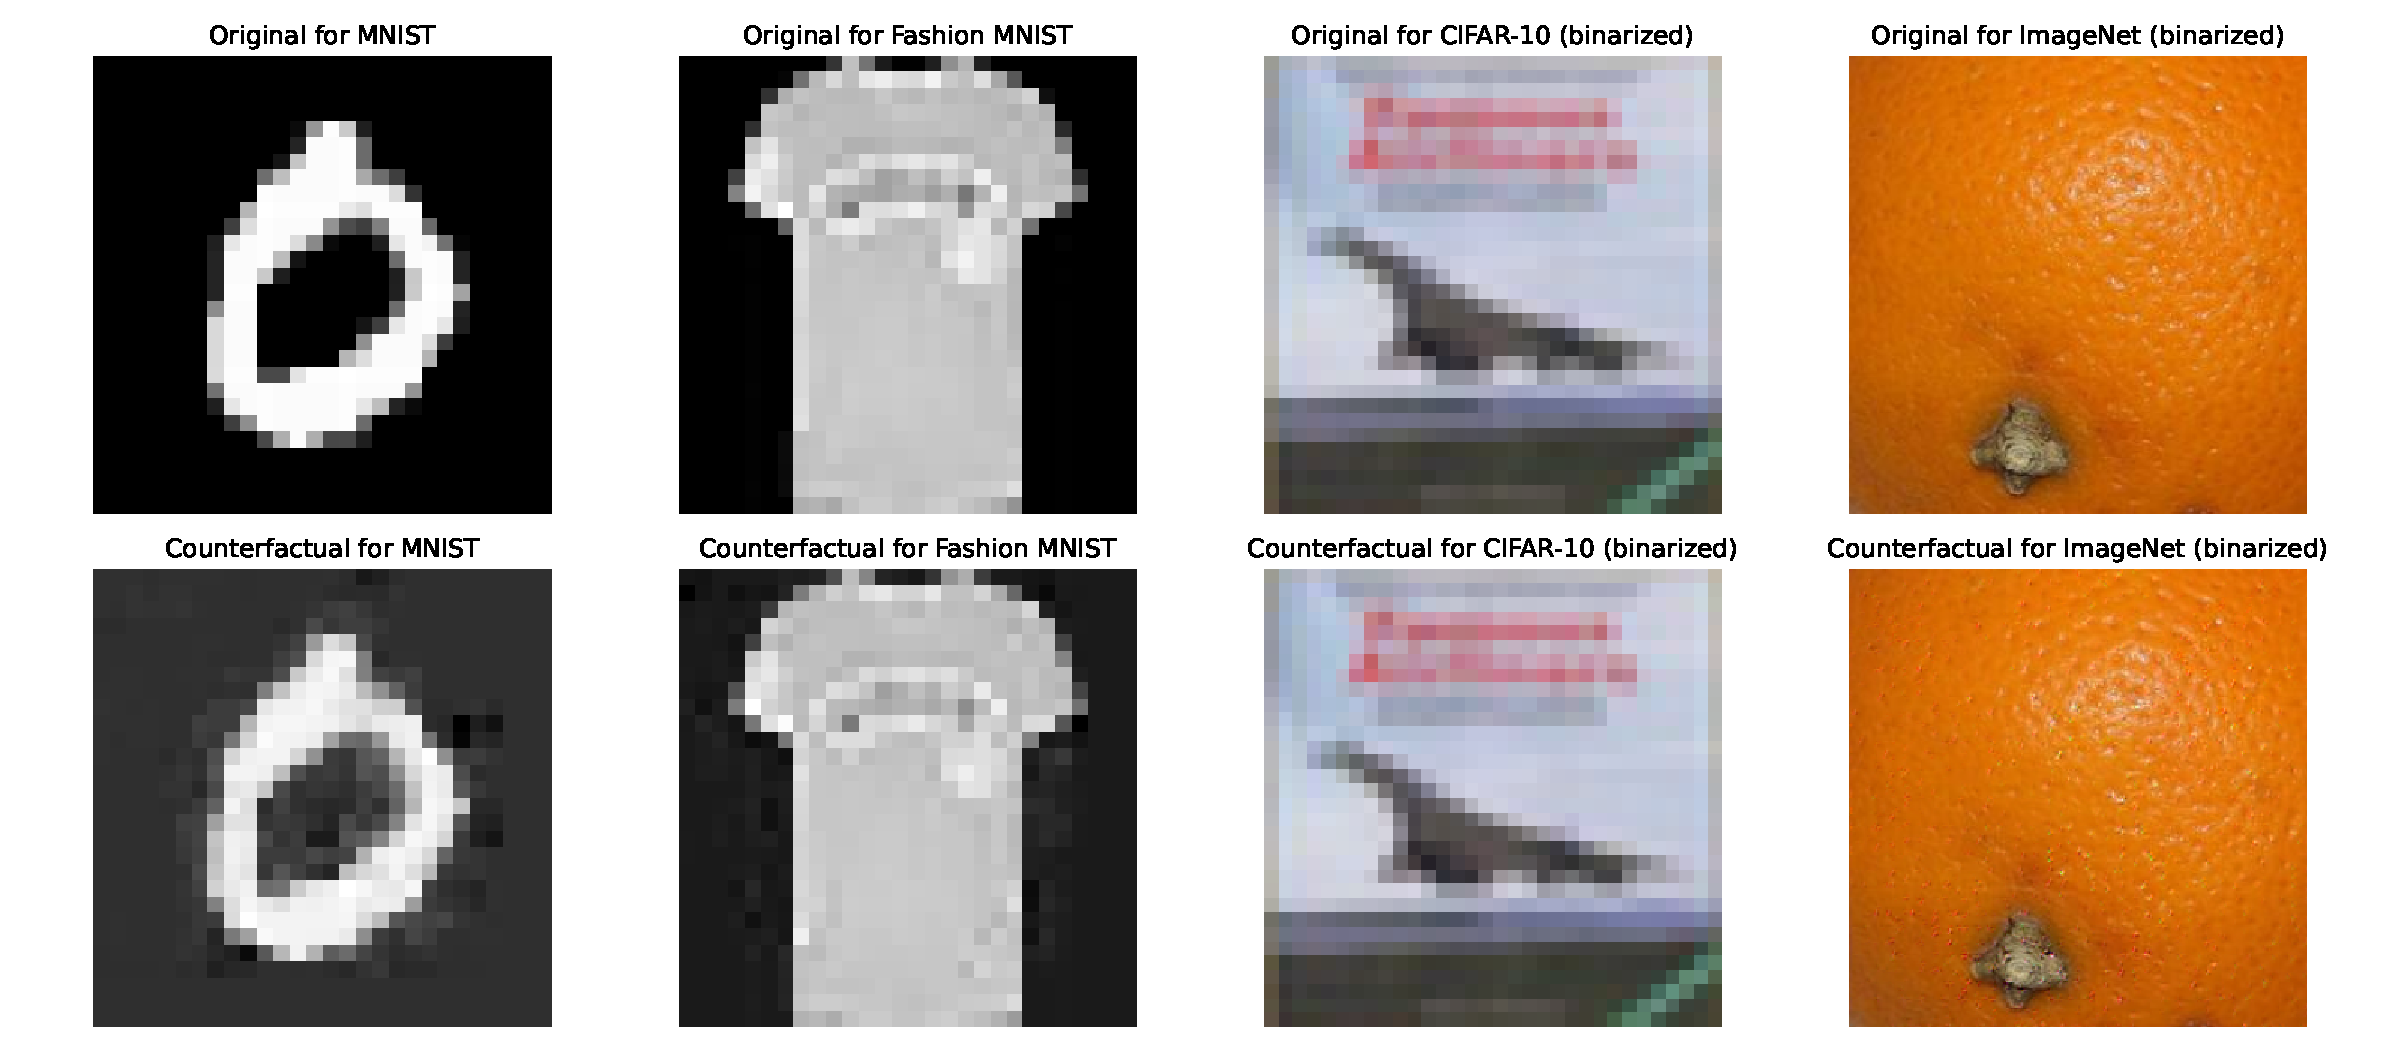
\includegraphics[width=\linewidth]{abb/counterfactual_examples.pdf}
    
    \caption{CEs for each experiment on the image data. In the top row, the original images are shown. In the bottom row the CEs are given.}
    \label{fig:examples_image}
\end{figure}
\noindent
To proof hypothesis 1, which stated that the average transferability rate has a negative correlation to the additional training epochs, the Spearman rank correlation and p-value can be calculated. These values are also given in the figure \ref{fig:add_epochs_image} for each experiment. The correlations are all negative which indicate a negative linear dependency. The corresponding p-values are very small and therefore show that the negative linear dependency is significant. \\
\begin{figure}[h]
    \centering 
    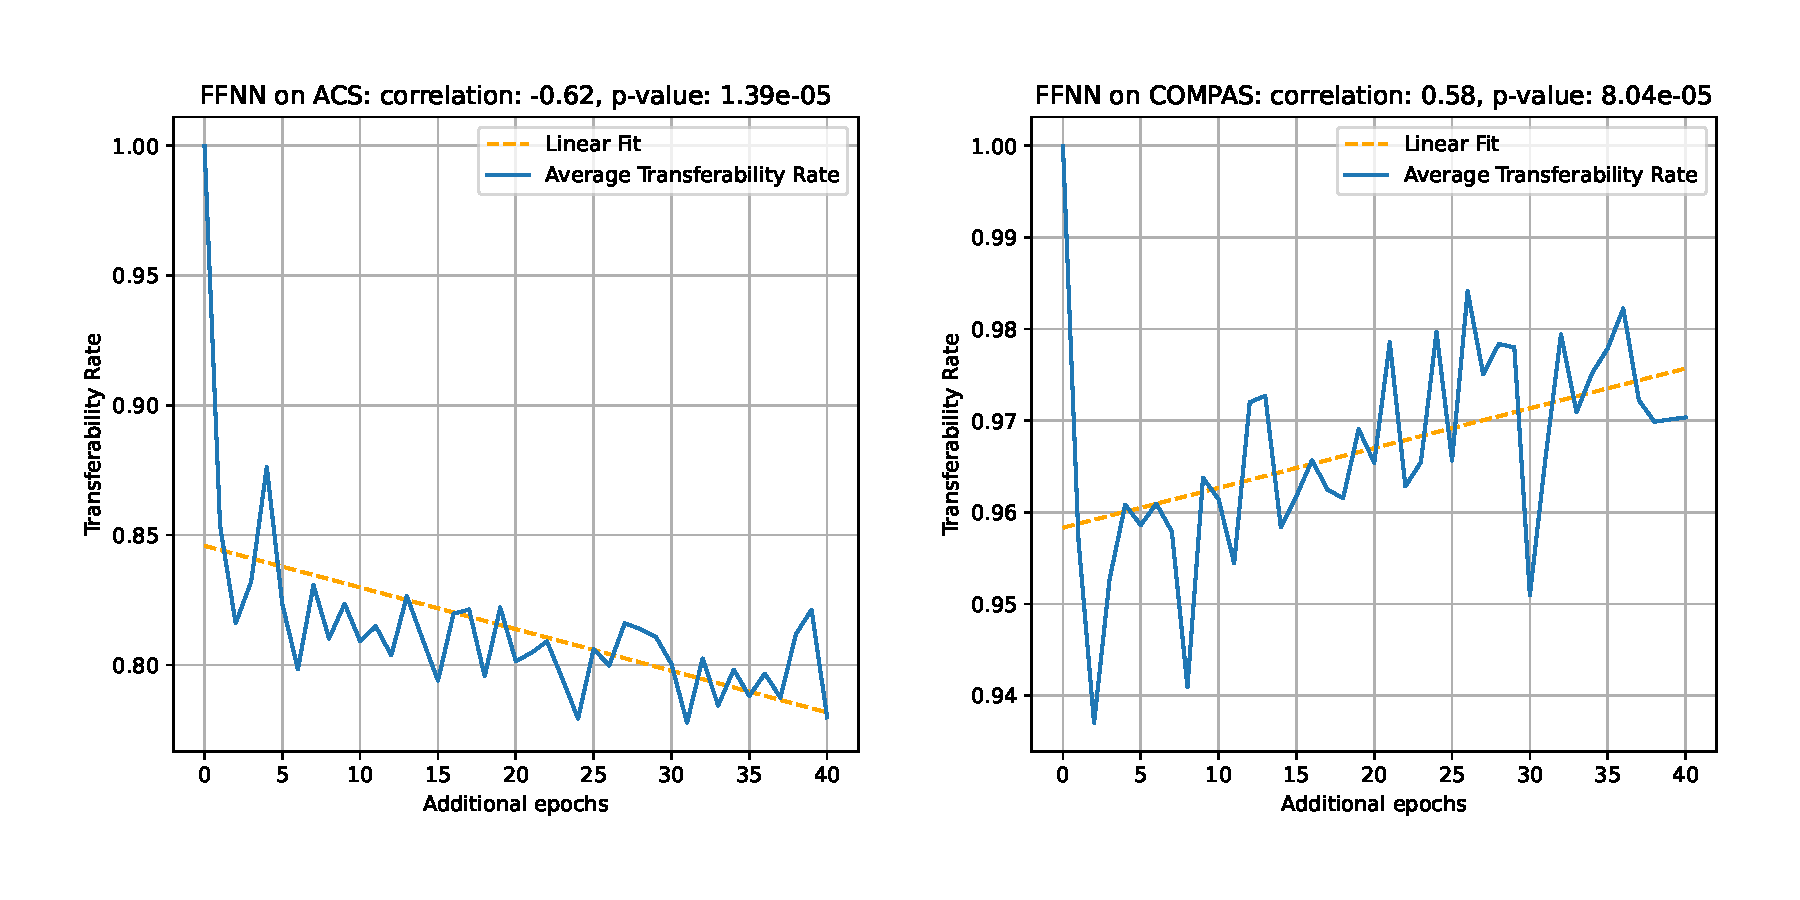
\includegraphics[width=\linewidth]{abb/epoch_evaluation_tabular.pdf}
    
    \caption{Average transferability rate for additional epochs on tabular datasets, FFNNs with different hyperparameters for number of layers and features were choosen to calculate the average over a bigger sample size.}
    \label{fig:add_epochs_tabular}
\end{figure}
\noindent
In figure \ref{fig:add_epochs_tabular}, the results of the same experiment using tabular data are shown. The \textit{ACS} dataset supports the earlier assumption from the image dataset that more training epochs lead to lower transferability. Interestingly, the COMPAS dataset shows the opposite trend. In this case, the transferability rate actually increases with more training epochs. Here’s a student-like rewrite of your sentence without special characters:

When looking at the Spearman rank correlations and p-values, the \textit{ACS} dataset shows a negative correlation with a p-value below 0.05. For \textit{COMPAS}, the positive correlation is also significant.\\

\subsection{Experiment 2: Base model vs. reference model with different number of parameters}
In this test, the transferability rate for different numbers of model parameters has been tested. Here, also different model architectures as \textit{K-SVM} or \textit{RF} can be evaluated. \\
For experiments run with neural networks a linear trend can be observed. The average transferability rates for neural networks of different complexities can be seen in figure \ref{fig:arch_eval_nns}. \\
\begin{figure}[h]
    \centering
    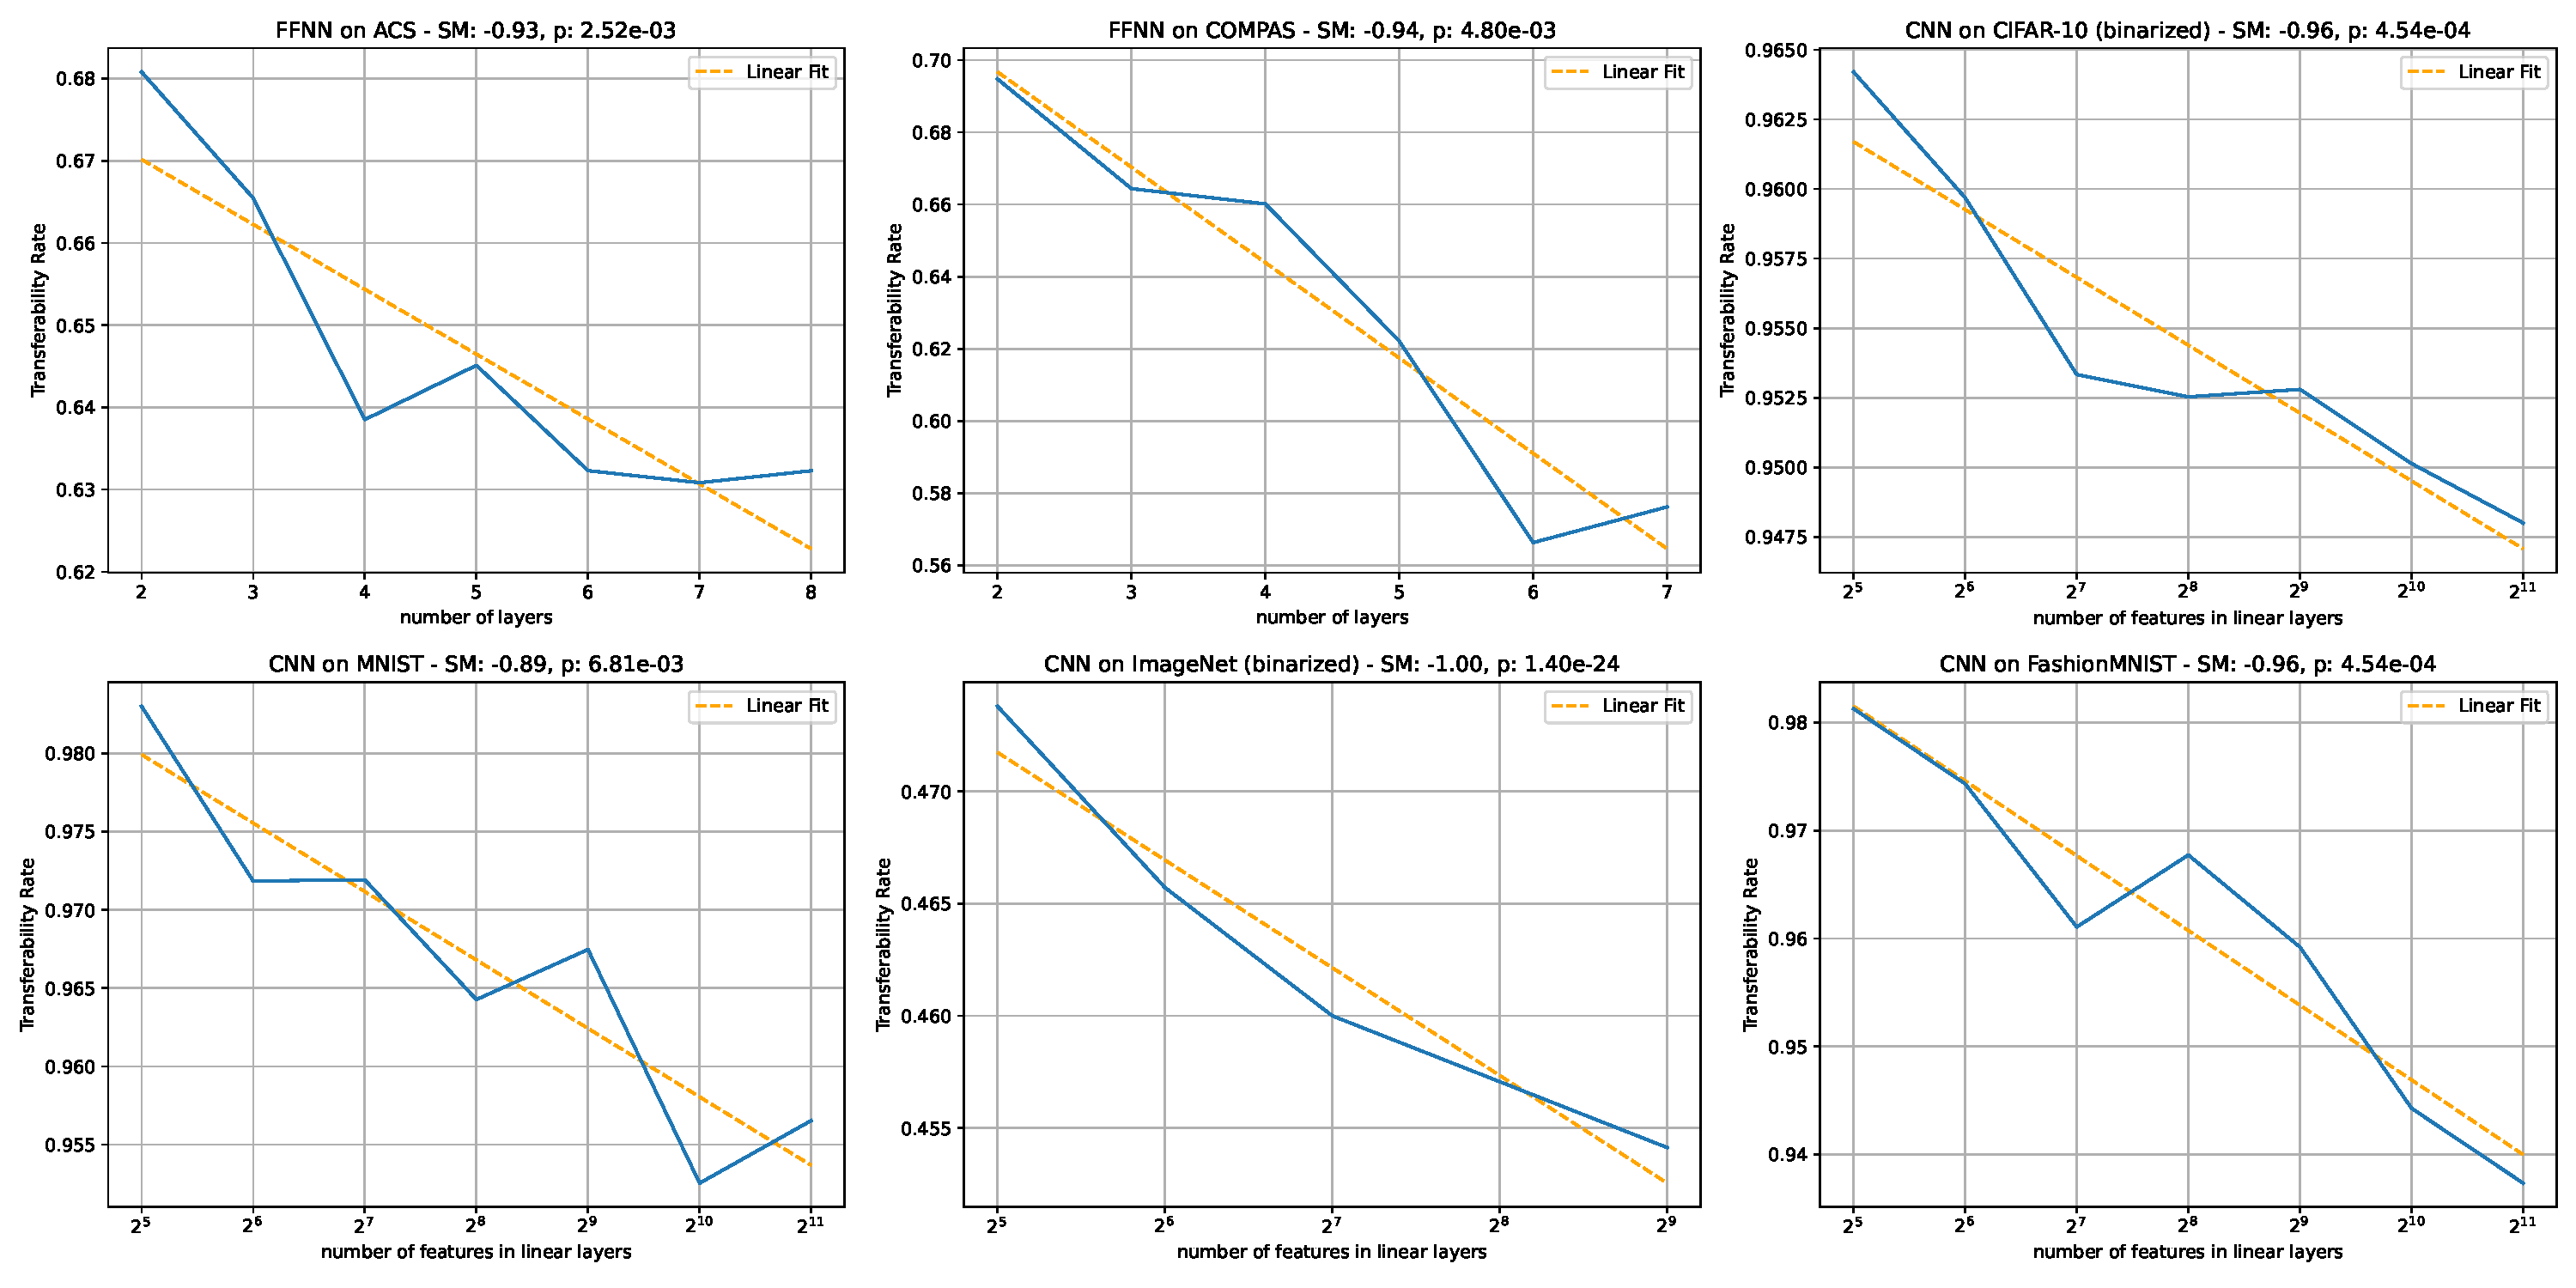
\includegraphics[width=\linewidth]{abb/architecture_evaluation_nns.pdf}
    \caption{Transferability rate for neural networks with different number of hyperparameters. Both the reference model and base model have the same architecture but were trained seperatly.}
    \label{fig:arch_eval_nns}
\end{figure}
\noindent
For both image and tabular data, with increasing model complexity the transferability rate decreases. Even the \textit{COMPAS} dataset, which has been a counterexample in the first experiment, shows a negative correlation. The curves of average transferability rate do have some bumps but the Spearman rank correlation and p-value indicate a strong negative correlation with statistical significance.\\
On tabular data, different model types have also been tested as they often outperform neural networks. For this experiment, RF and K-SVM with polynomial kernel have been choosen as a representation of all different model approaches. The experiment's results are illustrated in figure \ref{fig:arch_eval_other}.\\
\begin{figure}[h]
    \centering
    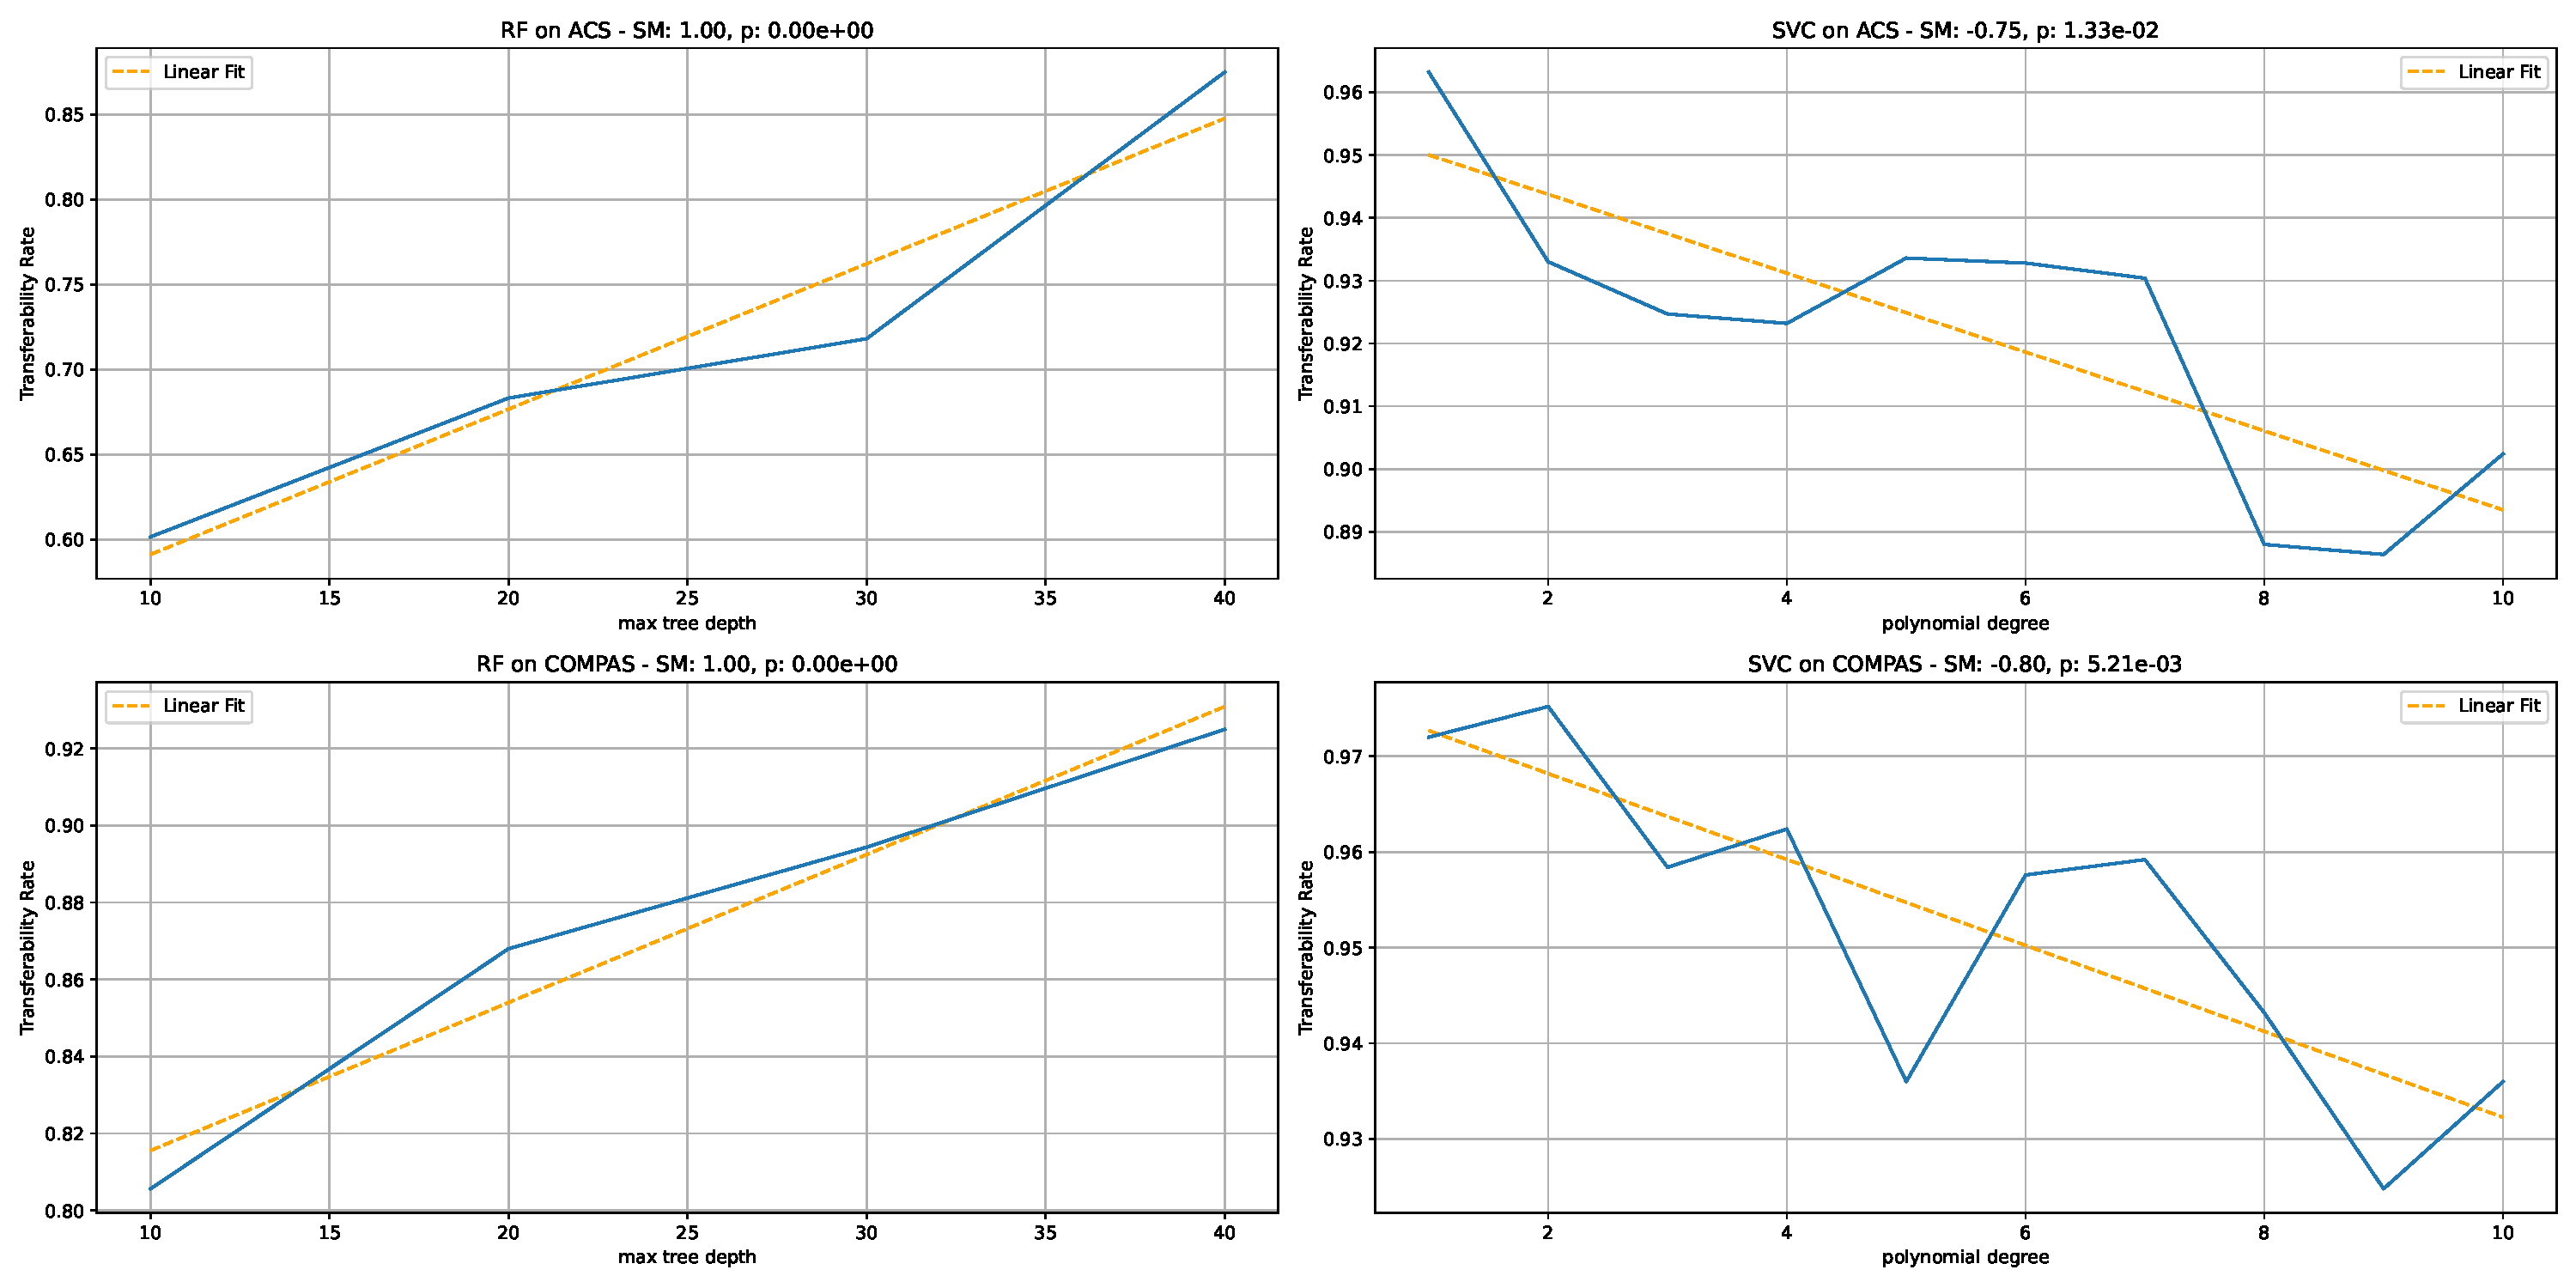
\includegraphics[width=\linewidth]{abb/architecture_evaluation_other_models.pdf}
    \label{fig:arch_eval_other}
    \caption{Transferability rate for RF and K-SVM. Both the reference model and base model have the same architecture but were trained seperatly.}
\end{figure}
\noindent
For RF a linear dependency can be observed eventough the correleation is positive. For deeper internal trees, the transferability rate increases. This holds true for both datasets. The Spearman rank correlation is 1 and the p-value is 0 which proof the positive linear dependency. \\
Kernelized SVM with a polynomial kernel however do have the same property as neural networks. For increasing model complexity, the average transferability rate decreases. This is emphasized by the correlation and the p-value being below the choosen threshold.

\section{Analysis}
In the previous section the experiments' results have been presented. Most of the experiments do proof the stated hypotheses from section \textit{Experiments}. \\
For neural networks, which are epoch-vise trained models, the statment \textit{"the transferability rate decreases as the number of additional epochs increases"} holds mostly true. Only for the experiment on the \textit{COMPAS} dataset, the opposite dependency has been detected. This effect might be given, because of the data distribution which could be different from the other datasets. When setting this aside, the p-values, which are all below 0.05, indicate a statistical significant negative correlation. Therefore, the first hypothesis is proofen eventough a deeper look into the \textit{COMPAS} dataset has to be taken in the future. \\
The second hypothesis is also proofen that for zero additional epochs, the transferability rate is one as this can be seen across all six experiments.\\
The evaluation on the model complexity also showed that more complex models have a lower transferability rate than models with a lower complextity. Here's a clearer, student-like version:

This is true for both neural networks and K-SVM, but for Random Forest, a positive correlation can be seen. Therefore, it cannot be concluded that a higher model complexity indicates a lower transferability rate. 

\section{Conclusion}
In this project, two experiments were done on multiple different datasets and different model architectures. The goal was to investigate whether CEs for a model also work for differnet models. As this is a very generic question and no previous work has been done, the experiments were designed to be very simple. The idea was to identify rules which apply to all model types and all dataset types.\\
Two main ideas were evaluated in this project which were formulated as hypotheses in the beginning. It has been shown, that at least for most tested datasets, the transferability rate decreases when the reference model is trained for additional epochs. It is also shown that more complex neural networks have a lower transferability rate than more complex ones. For RF models, the opposite dependency is shown while polynomial SVMs have a similar dependency as neural networks. \\
The experiments showed, that CEs are transferable across different models. However, the number of transferable counterfactuals decreases even for small changes in the model. \\
Eventhough trends have been found, the experiments were very limited. First of all, for simplicity all datasets were converted to binary labels. This makes it easy to generate counterfacutal examples as the label just has to be inverted. When generating CEs on multilabel datasets, more than one optional counterfactual label is available. \\
For tabular data, it is common to have continuous values for example a person's income or age but also binary values like the gender or mariage status. When generating the counterfactual example, simply the \textit{Cross Entropy Loss} \cite{mao2023crossentropylossfunctionstheoretical} is used. Therefore, binary values are handled like continuous values and could be changed to 0.57 for example. This leads to unrealistic datapoints. It could be easily handled by modifying the loss function but would lead to more complex experiment setups as each feature needs manual handling.For image data, a similar problem comes up because the pixel values range from 0 to 1. However, this was handled during the generation of counterfactual examples by penalizing values outside that range and clipping the pixel values to stay between 0 and 1 after convergence.\\
To generate many different datapoints which were used to calculate an average, the experiments were run multiple times per datapoint. This results to long runtimes for each epoch, especially for K-SVM models because they are not optimized for GPU. It would be interesting to test even more models and datasets to see if the stated assumption are emphasized.\\
Apart from more data for the described experiments, next steps would take into account different model architectures. For all done tests, the base and reference model have the same number of layers, features, etc.An interesting direction for future research is to examine how the transferability rate changes as the difference between two models increases. It remains to be explored whether the transferability consistently decreases with greater distance between models and whether the same effect appears when comparing different model architectures.\\ 
\newpage
\bibliographystyle{plain}
\bibliography{references}


\newpage
\appendix

\section{Usage of AI tools}
In this project, AI tools were used. For the coding part mainly GitHub Copilot was used for code completiton. It was mainly used to complete code lines are to complete configs as they are often repetitive. I had trouble with the \textit{dice-ml} library which I used to generate CEs for non-differentiable models. The library is not well documented and therefore I used Copilot for the correct usage of the library. The rest of the code was written by myself or was already given by some excercises from the lecture.\\
For research work, ChatGPT has been used to summarize two extensive papers I found on the topic of CEs.\\
Additionally, a few sentences were rewritten by ChatGPT as I had trouble with the wording. This only applies to a few sentences in the introduction and the related work section as well as in the conclusion. The rest of the report was written by myself.\\

\section{Statutory Declaration}
I officially ensure, that this paper has been written solely on my own. I herewith officially ensure, that I have not used any other sources but those stated by me. Any and every parts of the text which constitute quotes in original wording or in its essence have been explicitly referred by me by using official marking and proper quotation. This is also valid for used drafts, pictures and similar formats.\\
\vspace{3cm}

\begin{tabbing}
    %rule length 6.8 to the end of the line
\rule{5cm}{0.4pt} \hspace{3cm} \rule{6cm}{0.4pt}\\
Ort, Datum \hspace{6.4cm} \= Unterschrift (Frederik Hüttemann)\\
\end{tabbing}

\end{document}

